\section{Economic Growth: Stylized Facts and the Solow Model}

%=====================================================================
\subsection{Growth facts and convergence \pg{68--69}}

\paragraph{Notation used for the facts.}
\begin{itemize}
  \item $Y_t$ = aggregate output (= aggregate income), $L_t$ = labour input (population, workers), $K_t$ = aggregate capital stock, $C_t$ = consumption, $I_t$ = investment, $w_t$ = real wage, $t$ = time.
  \item Lower-case letters are \emph{per capita} (per worker): $y_t = Y_t/L_t$ (income per capita), $k_t=K_t/L_t$, $c_t = C_t/L_t$, $i_t = I_t/L_t$.
  \item A dot over a variable is its time derivative, $\dot X_t = dX_t/dt$; so $\dot X_t/X_t$ is the (instantaneous) \emph{growth rate} of $X$.
  \item \textbf{Labour share of output} $= \dfrac{w_tL_t}{Y_t}$: the fraction of total income paid to workers. In the data it is roughly constant over time.
\end{itemize}

\paragraph{Why the facts matter.} The stylized growth facts are the yardstick used to evaluate a growth model: we build the Solow model and then ask whether the variables in the model behave like the variables in the data (Section~\ref{sec:sol-eval}). Facts 1--4 describe an economy in the \emph{long run}, i.e.\ after economic development has taken place. Facts 5--7 describe features of the \emph{development process} across countries.

\begin{enumerate}
  \item \textbf{Steady growth.} Income per capita $y=Y/L$ grows at a (roughly) constant rate.
  \item \textbf{Balanced growth.} Consumption $C$ and investment $I$ grow, on average, at the same rate as output $Y$ (so the shares $C/Y$ and $I/Y$ are stable).
  \item \textbf{Capital deepening.} The capital stock $K$ grows at a constant rate that is greater than the growth rate of the labour input $L$ (so capital per worker $k$ rises over time).
  \item \textbf{Stable return.} The rate of return to capital is (roughly) constant.
  \item \textbf{Large cross-country differences} in (a) income \emph{levels} (a 20-fold gap between rich and poor countries is not uncommon) and (b) \emph{growth rates}:
  \begin{itemize}
    \item average performance: Canada, U.S.: $\dot y/y\approx 2\%$ per year;
    \item growth miracles: $\dot y/y\approx 5\%$ per year for long periods (Hong Kong, Japan);
    \item growth disasters: long periods of stagnation or decline (e.g.\ Argentina).
  \end{itemize}
  \item \textbf{No general catch-up.} Across all countries there is a (weak) tendency for rich countries to grow faster, so poor countries become relatively poorer.
  \item \textbf{Catch-up among similar countries.} Within the group of rich countries (OECD), the poorest ones grow the fastest.
\end{enumerate}

\begin{keybox}[title=Absolute vs.\ conditional convergence]
\begin{itemize}
  \item \textbf{Absolute convergence:} the hypothesis that \emph{all} poor countries grow faster than rich ones and therefore catch up in per-capita income. \emph{Not supported by the data} (fact 6).
  \item \textbf{Conditional convergence:} the hypothesis that only \emph{similar} countries converge, i.e.\ countries with similar technologies and similar economic policies (saving rates, population growth). Each country converges to its \emph{own} long-run path. \emph{Supported by the data} (fact 7).
\end{itemize}
\end{keybox}

%=====================================================================
\subsection{The Solow model: setup and equations \pg{1}}

\paragraph{Setup.}
\begin{itemize}
  \item \textbf{Environment:} continuous time $t\ge 0$; closed economy; one good, used both for consumption and as capital.
  \item \textbf{Variables} (all functions of $t$): output $Y_t$, capital $K_t$, labour $L_t$, technology (labour efficiency) $A_t$, consumption $C_t$, investment $I_t$, rental rate of capital $r_t$, real wage $w_t$. The product $A_tL_t$ is \emph{effective labour}: the number of workers times the efficiency of each worker.
  \item \textbf{Parameters} (constants):
  \begin{itemize}
    \item $\alpha\in(0,1)$: capital's exponent in production (= capital share of income, see below);
    \item $s\in[0,1]$: saving rate, the fixed fraction of output that is saved and invested;
    \item $\delta>0$: depreciation rate of capital;
    \item $n\ge 0$: population growth rate, $\dot L_t/L_t = n$;
    \item $x\ge 0$: growth rate of technology, $\dot A_t/A_t = x$.
  \end{itemize}
  \item \textbf{Key behavioural assumption:} there is no optimization by households; they simply save the exogenous fraction $s$ of output. Firms are competitive: they take $r_t$ and $w_t$ as given. $s,n,x,\delta$ are \emph{exogenous}.
  \item \textbf{Production} is Cobb--Douglas with \emph{labour-augmenting} technology: $Y_t=(A_tL_t)^{1-\alpha}K_t^{\alpha}$. It has constant returns to scale (exponents sum to $1$) and diminishing marginal returns to capital ($\alpha<1$).
  \item \textbf{Three ways to measure a variable $X$:}
  \begin{itemize}
    \item aggregate: $X_t$ (capital letter);
    \item per capita: lower case, e.g.\ $y_t = Y_t/L_t$, $k_t=K_t/L_t$, $c_t=C_t/L_t$, $i_t = I_t/L_t$;
    \item per effective worker (``hat''): $\hat y_t = \dfrac{Y_t}{A_tL_t}$, $\hat k_t = \dfrac{K_t}{A_tL_t}$, $\hat c_t = \dfrac{C_t}{A_tL_t}$, $\hat i_t = \dfrac{I_t}{A_tL_t}$.
  \end{itemize}
  The two normalized measures are linked by $y_t = A_t\hat y_t$, $k_t = A_t\hat k_t$, etc.
\end{itemize}

\paragraph{Calculus rules used below.}
\begin{itemize}
  \item Quotient rule: $\dfrac{d}{dt}\Big(\dfrac{u}{v}\Big) = \dfrac{\dot u v - u\dot v}{v^2}$. \quad Product rule: $\dfrac{d}{dt}(uv) = \dot u v + u\dot v$.
  \item Chain rule: $\dfrac{d}{dt}f(u_t) = f'(u_t)\,\dot u_t$; in particular $\dfrac{d}{dt}\ln X_t = \dfrac{\dot X_t}{X_t}$ (the growth rate).
  \item Hence for $Z = X^aW^b/V$: $\ \dfrac{\dot Z}{Z} = a\dfrac{\dot X}{X}+b\dfrac{\dot W}{W}-\dfrac{\dot V}{V}$ (take logs, then differentiate).
\end{itemize}

\paragraph{The model in three forms.}
\begin{center}
\renewcommand{\arraystretch}{1.35}
\begin{tabular}{lllc}
\textbf{Aggregate} & \textbf{Per capita} & \textbf{Per effective worker} & \\ \hline
$Y_t=(A_tL_t)^{1-\alpha}K_t^{\alpha}$ & $y_t=A_t^{1-\alpha}k_t^{\alpha}$ & $\hat y_t=\hat k_t^{\alpha}$ & (M1)\\
$Y_t=C_t+I_t$ & $y_t=c_t+i_t$ & $\hat y_t=\hat c_t+\hat i_t$ & (M2)\\
$I_t=sY_t$ & $i_t=sy_t$ & $\hat i_t=s\hat y_t$ & (M3)\\
$\dot K_t=I_t-\delta K_t$ & $\dot k_t=i_t-(\delta+n)k_t$ & $\dot{\hat k}_t=\hat i_t-(\delta+n+x)\hat k_t$ & (M4)\\
 & & $r_t=\alpha\hat k_t^{\alpha-1}$ & (M5)\\
 & & $w_t=(1-\alpha)A_t\hat k_t^{\alpha}$ & (M6)
\end{tabular}
\end{center}
(M1) is technology, (M2) the goods-market (resource) constraint, (M3) the saving rule, (M4) capital accumulation, (M5)--(M6) the competitive factor prices.

\paragraph{Deriving the per-capita and per-effective-worker forms of (M1).}
Divide the aggregate production function by $L_t$:
\begin{align*}
y_t=\frac{Y_t}{L_t} &= \frac{A_t^{1-\alpha}L_t^{1-\alpha}K_t^{\alpha}}{L_t} && \text{(expand $(A_tL_t)^{1-\alpha}$)}\\
&= A_t^{1-\alpha}L_t^{-\alpha}K_t^{\alpha} && \text{($L^{1-\alpha}/L = L^{-\alpha}$)}\\
&= A_t^{1-\alpha}\Big(\frac{K_t}{L_t}\Big)^{\alpha} = A_t^{1-\alpha}k_t^{\alpha}.
\end{align*}
Divide instead by effective labour $A_tL_t$:
\begin{align*}
\hat y_t = \frac{Y_t}{A_tL_t} &= (A_tL_t)^{1-\alpha-1}K_t^{\alpha} = (A_tL_t)^{-\alpha}K_t^{\alpha} = \Big(\frac{K_t}{A_tL_t}\Big)^{\alpha} = \hat k_t^{\alpha}.
\end{align*}
(M2)--(M3) follow by dividing both sides by $L_t$ or by $A_tL_t$ (they are linear, so the form is unchanged).

\textit{Interpretation:} because of constant returns to scale, output per effective worker depends only on capital per effective worker. Note that $A$ does \emph{not} appear in $\hat y=\hat k^\alpha$; this matters for the technology experiments below.

\paragraph{Deriving the per-capita accumulation equation in (M4).} Start from $k_t=K_t/L_t$ and use the quotient rule:
\begin{align*}
\dot k_t &= \frac{\dot K_tL_t - K_t\dot L_t}{L_t^2} && \text{(quotient rule)}\\
&= \frac{\dot K_t}{L_t} - \frac{K_t}{L_t}\cdot\frac{\dot L_t}{L_t} && \text{(split the fraction)}\\
&= \frac{I_t-\delta K_t}{L_t} - k_t\, n && \text{(aggregate (M4); $\dot L/L=n$)}\\
&= i_t-\delta k_t - nk_t = i_t-(\delta+n)k_t .
\end{align*}

\paragraph{Deriving the per-effective-worker accumulation equation in (M4).} Start from $\hat k_t = K_t/(A_tL_t)$; the denominator $A_tL_t$ has derivative $\dot A_tL_t+A_t\dot L_t$ (product rule):
\begin{align*}
\dot{\hat k}_t &= \frac{\dot K_t\,A_tL_t - K_t(\dot A_tL_t + A_t\dot L_t)}{(A_tL_t)^2} && \text{(quotient rule)}\\
&= \frac{\dot K_t}{A_tL_t} - \frac{K_t}{A_tL_t}\Big(\frac{\dot A_tL_t}{A_tL_t}+\frac{A_t\dot L_t}{A_tL_t}\Big) && \text{(split the fraction)}\\
&= \frac{\dot K_t}{A_tL_t} - \hat k_t\Big(\frac{\dot A_t}{A_t}+\frac{\dot L_t}{L_t}\Big) && \text{(cancel)}\\
&= \frac{I_t-\delta K_t}{A_tL_t} - \hat k_t(x+n) && \text{(aggregate (M4))}\\
&= \hat i_t - \delta\hat k_t - (x+n)\hat k_t = \hat i_t-(\delta+n+x)\hat k_t .
\end{align*}
\textit{Interpretation:} $(\delta+n+x)\hat k_t$ is \emph{break-even investment}: the investment needed just to keep $\hat k$ constant. Capital per effective worker is eroded by depreciation ($\delta$), by new workers who must be equipped ($n$), and by rising worker efficiency, which raises the number of effective workers ($x$).

\paragraph{Factor prices (M5)--(M6).} A competitive firm chooses $K_t$ and $L_t$ to maximize profit $Y_t - r_tK_t - w_tL_t$, taking $r_t,w_t$ as given. The first-order conditions set each price equal to the marginal product. Use $K_t=\hat k_t A_tL_t$ and $Y_t = \hat y_tA_tL_t$.
\begin{align*}
r_t = \frac{\partial Y_t}{\partial K_t} &= \alpha(A_tL_t)^{1-\alpha}K_t^{\alpha-1} && \text{(differentiate (M1) w.r.t.\ $K$)}\\
&= \alpha\frac{Y_t}{K_t} && \text{(multiply and divide by $K_t$)}\\
&= \alpha\frac{\hat y_tA_tL_t}{\hat k_tA_tL_t} = \alpha\frac{\hat y_t}{\hat k_t} && \text{(cancel $A_tL_t$)}\\
&= \alpha\frac{\hat k_t^{\alpha}}{\hat k_t} = \alpha\hat k_t^{\alpha-1}.
\end{align*}
\begin{align*}
w_t = \frac{\partial Y_t}{\partial L_t} &= (1-\alpha)A_t^{1-\alpha}L_t^{-\alpha}K_t^{\alpha} && \text{(differentiate (M1) w.r.t.\ $L$)}\\
&= (1-\alpha)\frac{Y_t}{L_t} && \text{(multiply and divide by $L_t$)}\\
&= (1-\alpha)A_t\frac{Y_t}{A_tL_t} = (1-\alpha)A_t\hat y_t = (1-\alpha)A_t\hat k_t^{\alpha}.
\end{align*}
\textit{Interpretation:} the return to capital depends only on $\hat k$ (diminishing returns: more capital per effective worker lowers $r$). The wage grows with technology $A$. Also $w_tL_t/Y_t = 1-\alpha$ and $r_tK_t/Y_t=\alpha$: factor shares are constant, matching the stable labour share in the data, and $w_tL_t+r_tK_t=Y_t$ (constant returns, so payments exhaust output).

\paragraph{The fundamental Solow equation.} Substitute the saving rule $\hat i_t=s\hat y_t$ (M3) and then $\hat y_t=\hat k_t^{\alpha}$ (M1) into (M4):
\begin{align*}
\dot{\hat k}_t &= \hat i_t-(\delta+n+x)\hat k_t = s\hat y_t-(\delta+n+x)\hat k_t ,
\end{align*}
\begin{keybox}[title=Fundamental equation of the Solow model]
\begin{equation}\label{eq:sol-fund}
\dot{\hat k}_t = \underbrace{s\hat k_t^{\alpha}}_{\text{actual investment}}-\underbrace{(\delta+n+x)\hat k_t}_{\text{break-even investment}} .
\end{equation}
\end{keybox}
$\hat k$ rises when actual investment per effective worker exceeds break-even investment, and falls otherwise. This one differential equation in $\hat k$ describes the whole economy: once we know $\hat k_t$, we get $\hat y_t=\hat k_t^\alpha$, $\hat c_t=(1-s)\hat y_t$, $r_t$, $w_t$, and all per-capita variables via $y_t=A_t\hat y_t$.

\paragraph{Explicit solution of \eqref{eq:sol-fund}.} We want $\hat k_t$ as a function of $t$, the parameters $(s,\delta,n,x,\alpha)$ and the initial value $\hat k_0$. Equation \eqref{eq:sol-fund} is nonlinear, but a change of variable makes it linear. Let $z_t = \hat k_t^{1-\alpha}$.
\begin{align*}
\dot z_t &= (1-\alpha)\hat k_t^{-\alpha}\dot{\hat k}_t && \text{(chain rule)}\\
&= (1-\alpha)\hat k_t^{-\alpha}\big[s\hat k_t^{\alpha}-(\delta+n+x)\hat k_t\big] && \text{(substitute \eqref{eq:sol-fund})}\\
&= (1-\alpha)\big[s-(\delta+n+x)\hat k_t^{1-\alpha}\big] && \text{(multiply out)}\\
&= (1-\alpha)\big[s-(\delta+n+x)z_t\big] = -\lambda\,(z_t - z^{*}),
\end{align*}
where $\lambda \equiv (1-\alpha)(\delta+n+x)$ and $z^{*}\equiv s/(\delta+n+x)$. A linear ODE $\dot z = -\lambda(z-z^*)$ has solution $z_t = z^*+(z_0-z^*)e^{-\lambda t}$ (check: differentiating gives $\dot z_t = -\lambda(z_0-z^*)e^{-\lambda t} = -\lambda(z_t-z^*)$). Substituting back $z=\hat k^{1-\alpha}$:
\begin{equation}\label{eq:sol-path}
\hat k_t^{1-\alpha}=\frac{s}{\delta+n+x}+\Big(\hat k_0^{1-\alpha}-\frac{s}{\delta+n+x}\Big)e^{-(1-\alpha)(\delta+n+x)t}.
\end{equation}
\textit{Interpretation:} the gap between $\hat k_t^{1-\alpha}$ and its long-run value shrinks at the constant exponential rate $\lambda=(1-\alpha)(\delta+n+x)$. As $t\to\infty$, $e^{-\lambda t}\to 0$, so $\hat k_t\to (s/(\delta+n+x))^{1/(1-\alpha)}$ from any $\hat k_0>0$.

%=====================================================================
\subsection{Steady state and the phase diagram \pg{2}}

\paragraph{Steady state.} A steady state (SS) is a value $\hat k^{*}$ at which $\hat k$ stops changing, $\dot{\hat k}=0$. Set \eqref{eq:sol-fund} to zero:
\begin{align*}
0 &= s(\hat k^{*})^{\alpha}-(\delta+n+x)\hat k^{*}\\
s(\hat k^{*})^{\alpha} &= (\delta+n+x)\hat k^{*} && \text{(move break-even term across)}\\
s &= (\delta+n+x)(\hat k^{*})^{1-\alpha} && \text{(divide by $(\hat k^*)^{\alpha}>0$)}\\
(\hat k^{*})^{1-\alpha} &= \frac{s}{\delta+n+x} && \text{(divide by $\delta+n+x$)}
\end{align*}
\begin{keybox}[title=Steady state]
\begin{equation}\label{eq:sol-kss}
\hat k^{*}=\Big(\frac{s}{\delta+n+x}\Big)^{\frac{1}{1-\alpha}},\qquad
\hat y^{*}=(\hat k^{*})^{\alpha}=\Big(\frac{s}{\delta+n+x}\Big)^{\frac{\alpha}{1-\alpha}},\qquad
\hat c^{*}=(1-s)\hat y^{*}.
\end{equation}
\end{keybox}
(We ignore the trivial SS $\hat k=0$.) Comparative statics: $\hat k^*$ and $\hat y^*$ rise with $s$ and fall with $\delta$, $n$ and $x$ (the exponent $1/(1-\alpha)$ is positive, so signs follow those of the ratio). A thriftier economy, or one with less capital dilution, has more capital per effective worker in the long run.

\begin{center}
\begin{tikzpicture}
\begin{axis}[width=8cm,height=5.2cm,axis lines=left,xmin=0,xmax=2.2,ymin=0,ymax=1.1,
  xtick={0.35,1,1.7},xticklabels={$\hat k^L$,$\hat k^{*}$,$\hat k^H$},ytick=\empty,
  xlabel={$\hat k_t$},ylabel={$\hat i_t$},clip=false]
\addplot[thick,blue,domain=0:2.1,samples=80]{0.5*x^0.4} node[right]{$s f(\hat k)=s\hat k^{\alpha}$};
\addplot[thick,red,domain=0:2.1]{0.5*x} node[right]{$(\delta+n+x)\hat k$};
\fill (axis cs:1,0.5) circle(1.5pt) node[above left]{SS};
\draw[dashed] (axis cs:1,0)--(axis cs:1,0.5);
\draw[dashed] (axis cs:0.35,0)--(axis cs:0.35,0.33);
\draw[dashed] (axis cs:1.7,0)--(axis cs:1.7,0.85);
\draw[-{Stealth},thick] (axis cs:0.45,0.03)--(axis cs:0.85,0.03);
\draw[-{Stealth},thick] (axis cs:1.6,0.03)--(axis cs:1.15,0.03);
\end{axis}
\end{tikzpicture}
\end{center}
\textbf{How to read the diagram.} The horizontal axis is capital per effective worker $\hat k_t$; the vertical axis measures investment per effective worker. The blue curve is actual investment $s\hat k^{\alpha}$: it starts at the origin, is steep for small $\hat k$ and flattens out because of diminishing returns ($\alpha<1$). The red line is break-even investment $(\delta+n+x)\hat k$, a straight ray through the origin. By \eqref{eq:sol-fund}, $\dot{\hat k}$ is the vertical distance between the two; the arrows on the axis show the direction in which $\hat k$ moves.

\begin{itemize}
  \item $\hat k_t<\hat k^{*}$ (e.g.\ $\hat k^L$, low capital stock): $s\hat k_t^{\alpha}>(\delta+n+x)\hat k_t\Rightarrow\dot{\hat k}_t>0$, so $\hat k$ rises.
  \item $\hat k_t=\hat k^{*}$: $s\hat k_t^{\alpha}=(\delta+n+x)\hat k_t\Rightarrow\dot{\hat k}_t=0$, so $\hat k$ does not change over time.
  \item $\hat k_t>\hat k^{*}$ (e.g.\ $\hat k^H$, high capital stock): $s\hat k_t^{\alpha}<(\delta+n+x)\hat k_t\Rightarrow\dot{\hat k}_t<0$, so $\hat k$ falls.
\end{itemize}
\textbf{Why the crossing is unique and stable.} Divide \eqref{eq:sol-fund} by $\hat k$: $\dot{\hat k}/\hat k = s\hat k^{\alpha-1}-(\delta+n+x)$. The term $s\hat k^{\alpha-1}$ is strictly decreasing in $\hat k$ (since $\alpha-1<0$), tends to $+\infty$ as $\hat k\to0$ and to $0$ as $\hat k\to\infty$. So it crosses the constant $\delta+n+x$ exactly once, at $\hat k^*$; it is above it to the left and below it to the right.

\textit{Interpretation:} the system converges to the SS from any starting point $\hat k_0>0$. $\hat k$ grows only during the \emph{transition} (e.g.\ from $\hat k^L$ to $\hat k^{*}$); once the economy is at $\hat k^*$, growth of $\hat k$ stops.

%=====================================================================
\subsection{Technology development: a one-time rise in \texorpdfstring{$A$}{A} \pg{2}}

\paragraph{Experiment.} The economy is in SS. At date $t_0$ the technology level jumps once from $A$ to $A'>A$; afterwards it again grows at rate $x$. $K$ and $L$ cannot jump (they are stocks), and $s,n,\delta,x$ are unchanged.

\paragraph{Direct (impact) effect.} Per-capita output is $y=A^{1-\alpha}k^{\alpha}$ by (M1). Since $k=K/L$ is unchanged at $t_0$, $y$ jumps up immediately by the factor $(A'/A)^{1-\alpha}$: the production function itself has improved.

\paragraph{Indirect effect.} Capital per effective worker $\hat k=K/(AL)$ has $A$ in the denominator, so it falls at $t_0$ to $\hat k_{t_0}=K/(A'L)<\hat k^{*}$. In the phase diagram the curves do \emph{not} move: $\hat y=\hat k^{\alpha}$ and the break-even line do not depend on the level of $A$, so $\hat k^{*}$ in \eqref{eq:sol-kss} is unchanged. The economy simply jumps \emph{left} along the $\hat k$ axis. It is pushed back into the transition region: $\dot{\hat k}>0$, capital accumulation speeds up, and $\hat k$ converges back to the same $\hat k^{*}$.

\paragraph{Long run.} On the BGP $y_t=A_t(\hat k^*)^{\alpha}$, so the new long-run path of $y$ is higher than the old one by the full factor $A'/A$. The impact jump delivers $(A'/A)^{1-\alpha}$; the remaining factor $(A'/A)^{\alpha}$ comes from the extra capital accumulated during the transition.

\begin{center}
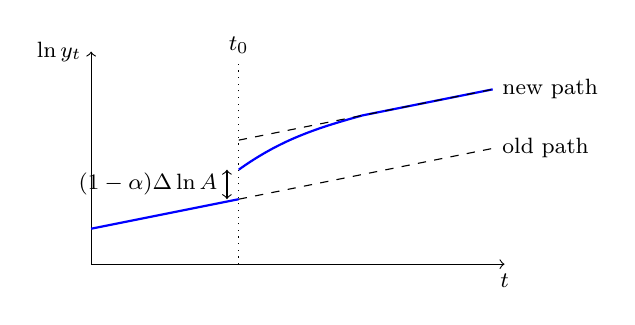
\begin{tikzpicture}[scale=0.75,every node/.style={font=\footnotesize}]
\draw[->](0,0)--(7,0) node[below]{$t$}; \draw[->](0,0)--(0,3.6) node[left]{$\ln y_t$};
\draw[dotted](2.5,0)--(2.5,3.4) node[above]{$t_0$};
\draw[thick,blue](0,0.6)--(2.5,1.1);
\draw[thick,blue](2.5,1.6) .. controls (3.2,2.1) and (3.8,2.3) .. (4.6,2.52)--(6.8,2.96);
\draw[dashed](2.5,1.1)--(6.8,1.96) node[right]{old path};
\draw[dashed](2.5,2.1)--(6.8,2.96);
\node[right] at (6.8,2.96){new path};
\draw[<->](2.3,1.1)--(2.3,1.6) node[midway,left]{$(1-\alpha)\Delta\ln A$};
\end{tikzpicture}
\end{center}
\textbf{How to read it.} The vertical axis is $\ln y$, so a constant growth rate shows up as a straight line with slope $x$. At $t_0$, $\ln y$ jumps by $(1-\alpha)\Delta\ln A$ (direct effect). It then grows faster than $x$ while $\hat k$ rebuilds (indirect effect), and finally runs along a new line of slope $x$ that lies $\Delta\ln A$ above the old one. The change in the level of $A$ has a level effect but no long-run growth effect.

%=====================================================================
\subsection{Evaluating the model against the growth facts \pg{3--5}}\label{sec:sol-eval}

Question: in the long run (and during transitions), do the variables of the Solow model behave like the variables in the data? Throughout we use \eqref{eq:sol-fund} and its growth-rate form
\begin{equation}\label{eq:sol-gk}
\frac{\dot{\hat k}_t}{\hat k_t}=s\hat k_t^{\alpha-1}-(\delta+n+x).
\end{equation}

\paragraph{Fact 1: in the long run, $y$ grows at the constant rate $x$.}
Step 1: relate growth of $y$ to growth of $\hat y$. Since $y_t=A_t\hat y_t$,
\begin{align*}
\frac{\dot y_t}{y_t} &= \frac{\dot A_t\hat y_t + A_t\dot{\hat y}_t}{A_t\hat y_t} && \text{(product rule)}\\
&= \frac{\dot A_t}{A_t} + \frac{\dot{\hat y}_t}{\hat y_t} = x + \frac{\dot{\hat y}_t}{\hat y_t}. \tag{F1a}
\end{align*}
Step 2: relate growth of $\hat y$ to growth of $\hat k$. Since $\hat y_t=\hat k_t^{\alpha}$,
\begin{align*}
\frac{\dot{\hat y}_t}{\hat y_t} &= \frac{\alpha\hat k_t^{\alpha-1}\dot{\hat k}_t}{\hat k_t^{\alpha}} && \text{(chain rule)}\\
&= \alpha\frac{\dot{\hat k}_t}{\hat k_t}. \tag{F1b}
\end{align*}
Because $\alpha$ is a constant, $\dot{\hat y}/\hat y$ depends only on $\dot{\hat k}/\hat k$.

Step 3: how does $\dot{\hat k}/\hat k$ change as the economy develops ($\hat k$ rises)? Differentiate \eqref{eq:sol-gk} with respect to $\hat k$:
\[
\frac{\partial(\dot{\hat k}/\hat k)}{\partial\hat k}=s(\alpha-1)\hat k^{\alpha-2}<0\qquad(\text{since }0<\alpha<1,\ s>0).
\]
Combined with (F1b), $\partial(\dot{\hat y}/\hat y)/\partial\hat k = \alpha s(\alpha-1)\hat k^{\alpha-2}<0$ as well.

Step 4: as $\hat k$ rises toward $\hat k^*$, the growth rates of $\hat k$ and $\hat y$ fall, reaching $0$ at the SS. Substituting into (F1a)--(F1b):
\[
\frac{\dot y_t}{y_t} = x+\alpha\frac{\dot{\hat k}_t}{\hat k_t}\ \longrightarrow\ x+\alpha\cdot 0 = x .
\]
\textit{Interpretation:} capital accumulation alone cannot sustain growth because of diminishing returns; in the long run per-capita income grows only because technology improves. The model reproduces fact 1, but the growth rate $x$ is exogenous (not explained).

\paragraph{Fact 2: balanced growth, $Y$, $C$, $I$ all grow at $x+n$.}
Write $Y_t=y_tL_t$ and take logs: $\ln Y_t=\ln y_t+\ln L_t$. Differentiate with respect to $t$:
\[
\frac{\dot Y_t}{Y_t}=\frac{\dot y_t}{y_t}+\frac{\dot L_t}{L_t}\ \longrightarrow\ x+n\quad\text{(long run, using fact 1)}.
\]
From (M2)--(M3), $C_t=(1-s)Y_t$ and $I_t=sY_t$. Taking logs, $\ln C_t=\ln(1-s)+\ln Y_t$; since $\ln(1-s)$ is a constant, its derivative is $0$, so $\dot C/C=\dot Y/Y=x+n$. In the same way $\dot I/I=\dot Y/Y=x+n$. The model displays balanced growth.

\paragraph{Fact 3: $K$ grows at a constant rate faster than $L$.}
Since $k_t=A_t\hat k_t$, by the product rule (as in (F1a))
\[
\frac{\dot k_t}{k_t}=\frac{\dot A_t}{A_t}+\frac{\dot{\hat k}_t}{\hat k_t} = x+\frac{\dot{\hat k}_t}{\hat k_t}\ \longrightarrow\ x \quad(\text{since } \dot{\hat k}/\hat k\to 0).
\]
Then $K_t=k_tL_t$ gives $\dot K/K=\dot k/k+n\to x+n$. This is constant, and it exceeds labour growth $n$ whenever $x>0$. So fact 3 holds as long as technology grows.

\paragraph{Fact 4: the rate of return to capital is constant.}
From (M5), $r_t=\text{MPK}=\alpha(A_tL_t)^{1-\alpha}K_t^{\alpha-1}=\alpha\hat k_t^{\alpha-1}$. The owner of capital earns $r_t$ but loses $\delta$ per unit through depreciation, so the net rate of return is
\[
r_t-\delta=\alpha\hat k_t^{\alpha-1}-\delta\ \longrightarrow\ \alpha(\hat k^*)^{\alpha-1}-\delta \quad\text{(long run)},
\]
a constant because $\hat k^*$ is constant. Similarly the labour share $w_tL_t/Y_t=1-\alpha$ is constant at all times.

\paragraph{Facts 6 and 7: conditional, not absolute, convergence.} The tools are:
(i) $y=A\hat y=A\hat k^{\alpha}$; (ii) $\dot y/y=x+\dot{\hat y}/\hat y$ (F1a); (iii) $\dot{\hat y}/\hat y=\alpha\,\dot{\hat k}/\hat k$ (F1b); (iv) $\dot{\hat k}/\hat k=s\hat k^{\alpha-1}-(\delta+n+x)$ \eqref{eq:sol-gk}; (v) $\partial(\dot{\hat k}/\hat k)/\partial\hat k<0$.
\begin{enumerate}[label=(\alph*)]
  \item \textbf{A country is poor because its $k=K/L$ is initially low, all parameters ($A$, $s$, $n$, $\delta$, $x$, $\alpha$) the same.}
  Low $k$ with the same $A$ means low $\hat k=k/A$, so by (i) $y$ is low. By (v), low $\hat k$ means a high $\dot{\hat k}/\hat k$, and by (ii)--(iii) a high $\dot y/y = x+\alpha\,\dot{\hat k}/\hat k$. The poor country is far below its SS, in its transition period, so it grows faster than the rich country. Both converge to the same $\hat k^*$ and the same path $y_t=A_t(\hat k^*)^{\alpha}$: \textbf{income convergence}.
  \item \textbf{A country is poor because its $A$ is low, all other parameters the same.}
  Both countries have the same $\hat k^*$ by \eqref{eq:sol-kss} (it does not depend on the level of $A$) and the same long-run growth rate $x$. In the long run $y^{P}_t/y^{R}_t = A^P_t(\hat k^*)^{\alpha}/(A^R_t(\hat k^*)^{\alpha}) = A^P/A^R<1$, a constant (both $A$'s grow at $x$). So the poor country \textbf{never catches up}: there is a permanent gap in income levels. During the transition, if the two countries start with similar $k$, the poor country has the \emph{higher} $\hat k=k/A$, hence by (v) the lower $\dot{\hat k}/\hat k$ and the lower $\dot y/y$: the relative gap widens (from $(A^P/A^R)^{1-\alpha}$ toward $A^P/A^R$) and then stays constant, while the absolute gap keeps growing at rate $x$.
  \item \textbf{Two countries have the same $y$ today, but one has a higher $s$ or a higher $x$.}
  Higher $s$ raises $\hat k^*$ \eqref{eq:sol-kss}, so the high-$s$ country is further below its SS and grows faster during the transition, toward a higher level path. Higher $x$ gives permanently faster long-run growth (fact 1). Either way the high-$s$/high-$x$ country grows faster: \textbf{divergence} from the same starting point.
\end{enumerate}
\textit{Conclusion:} the Solow model predicts convergence only among countries with similar parameters (conditional convergence, fact 7). Since not all countries are alike (poor countries may have lower $s$, $A$, or $x$), we should not expect a general narrowing of income gaps (no absolute convergence, fact 6).

\paragraph{Fact 5: large differences in income levels; growth miracles and disasters.}
On the BGP, combining $y_t=A_t\hat y^*$ with \eqref{eq:sol-kss},
\[
y_t = A_t\Big(\frac{s}{\delta+n+x}\Big)^{\frac{\alpha}{1-\alpha}} .
\]
Level differences can therefore come from differences in the technology level $A$ and, to some extent, the saving rate $s$. ``To some extent'': with $\alpha=1/3$ the exponent is $\alpha/(1-\alpha)=1/2$, so even a 4-fold difference in $s$ produces only a 2-fold difference in $y$. A 20-fold gap must therefore come mostly from $A$.

\emph{Speed of convergence.} How long can transitional growth last? Write \eqref{eq:sol-gk} in terms of $\ln\hat k$ and take a first-order Taylor expansion around $\ln\hat k^*$ (log-linearization: $f(u)\approx f(u^*)+f'(u^*)(u-u^*)$):
\begin{align*}
\frac{d\ln\hat k_t}{dt} &= s\,e^{-(1-\alpha)\ln\hat k_t}-(\delta+n+x) && \text{(since $\hat k^{\alpha-1}=e^{(\alpha-1)\ln\hat k}$)}\\
&\approx 0 - (1-\alpha)s(\hat k^*)^{\alpha-1}(\ln\hat k_t-\ln\hat k^*) && \text{(Taylor; value at SS is 0)}\\
&= -(1-\alpha)(\delta+n+x)(\ln\hat k_t-\ln\hat k^*) && \text{(SS: $s(\hat k^*)^{\alpha-1}=\delta+n+x$)}.
\end{align*}
So the log-gap to the SS closes at rate $\lambda=(1-\alpha)(\delta+n+x)$, the same $\lambda$ as in \eqref{eq:sol-path}. With $\alpha=1/3$ and $\delta+n+x=0.06$, $\lambda=0.04$: half of the gap closes in about $\ln 2/0.04\approx 17$ years. Transitional growth fades quickly as the SS is approached.

\begin{itemize}
  \item \textbf{Growth miracle} (5\% for decades): transitional growth cannot be sustained for long unless convergence is very slow, which requires a very high $\alpha$ (close to $1$, so $\lambda$ is small); otherwise it requires a high technology growth rate $x$.
  \item \textbf{Growth disaster:} requires a very low (or negative) value of $x$.
\end{itemize}

\begin{keybox}[title=Solow scorecard]
\begin{itemize}
  \item Long run: $\dot y/y=\dot k/k=x$; $\ \dot Y/Y=\dot C/C=\dot I/I=\dot K/K=x+n$; $\ r-\delta$ and factor shares constant. Facts 1--4 are reproduced.
  \item Predicts \emph{conditional} convergence (facts 6--7).
  \item Level differences come mainly from $A$ (and partly $s$); sustained growth comes only from the exogenous $x$, which the model does not explain.
\end{itemize}
\end{keybox}

%=====================================================================
\subsection{Welfare: the golden rule and dynamic (in)efficiency \pg{5--6}}

\paragraph{Setup.} Suppose a planner can choose the saving rate $s$ once and for all. Each $s$ gives a SS $\hat k^{ss}(s)$ via \eqref{eq:sol-kss}. Objective: find the $\hat k$ (and the $s$ that delivers it) that maximizes steady-state consumption per effective worker $\hat c^{ss}$. This is the \textbf{golden rule}.

\paragraph{Steady-state consumption as a function of $\hat k$.} In SS actual investment equals break-even investment, $\hat i^{ss}=s\hat y^{ss}=(\delta+n+x)\hat k^{ss}$, and $\hat y^{ss}=(\hat k^{ss})^{\alpha}$. Using (M2):
\begin{align*}
\hat c^{ss} &= \hat y^{ss}-\hat i^{ss} && \text{(M2)}\\
&= (\hat k^{ss})^{\alpha}-(\delta+n+x)\hat k^{ss}. && \text{(substitute SS values)}
\end{align*}

\paragraph{Maximizing.} Treat $\hat k$ as the choice variable:
\begin{align*}
\frac{\partial\hat c^{ss}}{\partial\hat k} &= \alpha\hat k^{\alpha-1}-(\delta+n+x)=0 && \text{(FOC)}\\
\alpha\hat k^{\alpha-1} &= \delta+n+x && \text{(i.e.\ $r=\delta+n+x$ by (M5))}\\
\hat k^{1-\alpha} &= \frac{\alpha}{\delta+n+x} && \text{(invert: $\hat k^{\alpha-1}=1/\hat k^{1-\alpha}$)}\\
\hat k_{gold} &= \Big(\frac{\alpha}{\delta+n+x}\Big)^{\frac{1}{1-\alpha}} .
\end{align*}
Second-order condition: $\partial^2\hat c^{ss}/\partial\hat k^2=\alpha(\alpha-1)\hat k^{\alpha-2}<0$, so this is a maximum. Since $\hat c^{ss}(\hat k)$ is concave, it is increasing for $\hat k<\hat k_{gold}$ and decreasing for $\hat k>\hat k_{gold}$.

\paragraph{Which saving rate delivers the golden rule?} Compare the two expressions
\[
\hat k^{ss}=\Big(\frac{s}{\delta+n+x}\Big)^{\frac1{1-\alpha}},\qquad
\hat k_{gold}=\Big(\frac{\alpha}{\delta+n+x}\Big)^{\frac1{1-\alpha}} .
\]
They are equal exactly when $s=\alpha$. Because $\hat k^{ss}$ is strictly increasing in $s$, $s>\alpha\Leftrightarrow\hat k^{ss}>\hat k_{gold}$ and $s<\alpha\Leftrightarrow\hat k^{ss}<\hat k_{gold}$.

\begin{center}
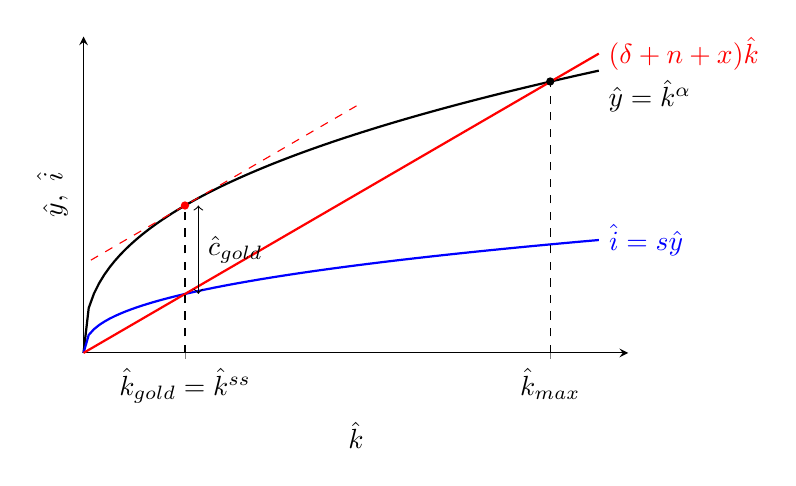
\begin{tikzpicture}
\begin{axis}[width=8.5cm,height=5.6cm,axis lines=left,xmin=0,xmax=3.7,ymin=0,ymax=1.85,
  xtick={0.689,3.17},xticklabels={$\hat k_{gold}=\hat k^{ss}$,$\hat k_{max}$},ytick=\empty,
  xlabel={$\hat k$},ylabel={$\hat y,\ \hat i$},clip=false]
\addplot[thick,black,domain=0:3.5,samples=100]{x^0.4};
\node[right] at (axis cs:3.5,1.5){$\hat y=\hat k^{\alpha}$};
\addplot[thick,blue,domain=0:3.5,samples=100]{0.4*x^0.4} node[right]{$\hat i=s\hat y$};
\addplot[thick,red,domain=0:3.5]{0.5*x};
\node[red,right] at (axis cs:3.5,1.75){$(\delta+n+x)\hat k$};
\addplot[dashed,red,domain=0.05:1.9]{0.862+0.5*(x-0.689)};
\fill[red] (axis cs:0.689,0.862) circle(1.5pt);
\fill (axis cs:3.17,1.587) circle(1.5pt);
\draw[dashed] (axis cs:0.689,0)--(axis cs:0.689,0.862);
\draw[dashed] (axis cs:3.17,0)--(axis cs:3.17,1.587);
\draw[<->] (axis cs:0.78,0.345)--(axis cs:0.78,0.862) node[midway,right]{$\hat c_{gold}$};
\end{axis}
\end{tikzpicture}
\end{center}
\textbf{How to read the diagram.} The black curve is output $\hat y$, the blue curve is investment $s\hat y$ and the red line is break-even investment. In SS, consumption $\hat c^{ss}$ is the vertical gap between $\hat y$ and the red line (because $\hat i^{ss}$ equals break-even investment). This gap is largest where the slope of $\hat y$ equals the slope of the red line, $\delta+n+x$: the dashed tangent touches $\hat y$ at $\hat k_{gold}$ and is parallel to the red line. The figure is drawn with $s=\alpha$, so the blue curve crosses the red line exactly at $\hat k_{gold}$. At $\hat k_{max}$ (where $\hat y$ meets the red line) all output must be invested to keep $\hat k$ constant ($s=1$) and consumption is zero.

\begin{keybox}[title=Golden rule and dynamic efficiency]
\[
\alpha\hat k_{gold}^{\alpha-1}=\delta+n+x\ \ (\text{i.e. } r-\delta=n+x),\qquad
\hat k_{gold}=\Big(\frac{\alpha}{\delta+n+x}\Big)^{\frac1{1-\alpha}},\qquad s_{gold}=\alpha .
\]
\begin{itemize}
  \item \textbf{Case 1, $s>\alpha$:} $\hat k^{ss}>\hat k_{gold}$. The economy is \textbf{dynamically inefficient}: lowering $s$ makes agents better off in \emph{all} periods.
  \item \textbf{Case 2, $0\le s<\alpha$:} $\hat k^{ss}<\hat k_{gold}$. The economy is \textbf{dynamically efficient}: changing $s$ involves a trade-off between periods, so no change is a Pareto improvement.
\end{itemize}
\end{keybox}
\textit{Interpretation of the golden rule condition:} at the golden rule the net return on capital $r-\delta$ equals the growth rate of the economy $n+x$. If $r-\delta<n+x$, there is ``too much'' capital: the extra output from the marginal unit of capital is less than what is needed just to maintain it.

\paragraph{Case 1 ($s>\alpha$): what happens if we lower $s$ to $\alpha$ at date $t_0$?}
\begin{enumerate}
  \item \textbf{$\hat k$ and $\hat y$.} Before $t_0$, $\dot{\hat k}=s\hat y-(\delta+n+x)\hat k=0$ at the old SS. At $t_0$, $s$ falls while $\hat k$ (a stock) cannot jump, so $s\hat y$ falls and $\dot{\hat k}<0$. $\hat k$ declines smoothly until it reaches the new SS, $\hat k_{gold}$. Since $\hat y_t=\hat k_t^{\alpha}$, $\hat y$ has the same shape.
  \item \textbf{$\hat c=(1-s)\hat y$.} At $t_0$, $\hat y$ is unchanged but $1-s$ rises, so $\hat c$ \emph{jumps up}. Afterwards $\hat c_t=(1-\alpha)\hat y_t$ falls with $\hat y$, settling at $\hat c_{gold}$. Since $\hat c^{ss}(\hat k)$ is maximized at $\hat k_{gold}$, $\hat c_{gold}>\hat c_{old}$. And since $\hat c_t$ declines monotonically toward $\hat c_{gold}$, it stays above $\hat c_{old}$ at every date. Consumption is higher in all periods: this is why $s>\alpha$ is inefficient.
  \item \textbf{$\hat i=s\hat y$.} At $t_0$, $\hat i$ jumps down (lower $s$, same $\hat y$), then declines further with $\hat y$ and levels off at the new SS.
\end{enumerate}
\begin{center}
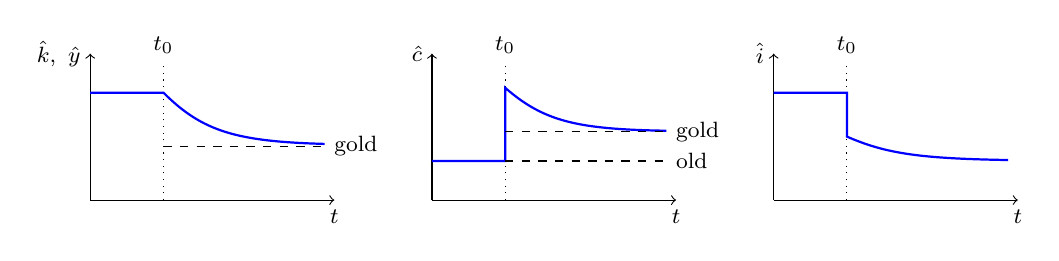
\begin{tikzpicture}[scale=0.62,every node/.style={font=\footnotesize}]
\draw[->](0,0)--(5,0) node[below]{$t$}; \draw[->](0,0)--(0,3) node[left]{$\hat k,\ \hat y$};
\draw[dotted](1.5,0)--(1.5,2.8) node[above]{$t_0$};
\draw[thick,blue](0,2.2)--(1.5,2.2) .. controls (2.3,1.4) and (3,1.2) .. (4.8,1.15);
\draw[dashed](1.5,1.1)--(4.8,1.1) node[right]{gold};
\begin{scope}[shift={(7,0)}]
\draw[->](0,0)--(5,0) node[below]{$t$}; \draw[->](0,0)--(0,3) node[left]{$\hat c$};
\draw[dotted](1.5,0)--(1.5,2.8) node[above]{$t_0$};
\draw[thick,blue](0,0.8)--(1.5,0.8)--(1.5,2.3) .. controls (2.3,1.6) and (3,1.45) .. (4.8,1.42);
\draw[dashed](1.5,0.8)--(4.8,0.8) node[right]{old};
\draw[dashed](1.5,1.4)--(4.8,1.4) node[right]{gold};
\end{scope}
\begin{scope}[shift={(14,0)}]
\draw[->](0,0)--(5,0) node[below]{$t$}; \draw[->](0,0)--(0,3) node[left]{$\hat i$};
\draw[dotted](1.5,0)--(1.5,2.8) node[above]{$t_0$};
\draw[thick,blue](0,2.2)--(1.5,2.2)--(1.5,1.3) .. controls (2.3,0.95) and (3,0.85) .. (4.8,0.82);
\end{scope}
\end{tikzpicture}
\end{center}
\textbf{How to read the panels.} Each panel plots one variable against time, with the policy change at $t_0$ (dotted line). Stocks ($\hat k$, and hence $\hat y$) move continuously; flows that depend directly on $s$ ($\hat c$, $\hat i$) jump at $t_0$ and then follow $\hat y$. In the middle panel the whole post-$t_0$ path of $\hat c$ lies above the old level.

\paragraph{Case 2 ($s<\alpha$): dynamic efficiency.} Here a change in $s$ creates a trade-off: it raises consumption and welfare in some periods but lowers it in others. For example, raising $s$ increases future $\hat k$ and output but reduces current $\hat c$ (see the next subsection); lowering $s$ raises $\hat c$ today but lowers it in the long run. No change in $s$ makes every period better off, so the allocation cannot be improved for all generations.

%=====================================================================
\subsection{Effects of a rise in \texorpdfstring{$s$}{s} (dynamically efficient region) \pg{8}}

\paragraph{Experiment.} The economy is in SS with $s_{old}<\alpha$. At $t_0$ the saving rate rises permanently to $s_{new}$ with $s_{old}<s_{new}\le\alpha$. All other parameters are unchanged; $\hat k$ cannot jump at $t_0$.

\begin{enumerate}
  \item \textbf{Growth rate of $\hat k$.} By \eqref{eq:sol-gk}, $\dot{\hat k}/\hat k=s\hat k^{\alpha-1}-(\delta+n+x)$. Before $t_0$ it equals $0$. At $t_0$, $s$ jumps up with $\hat k$ fixed, so $\dot{\hat k}/\hat k$ jumps up to a positive value. As $\hat k$ then rises, $s_{new}\hat k^{\alpha-1}$ falls, so $\dot{\hat k}/\hat k$ decays back to $0$.
  \item \textbf{Level of $\hat k$.} $\hat k$ rises, at a slowing pace, to a higher plateau. The new SS solves $s_{new}\hat k^{\alpha}=(\delta+n+x)\hat k$, so by \eqref{eq:sol-kss} $\hat k^{ss}_{new}=(s_{new}/(\delta+n+x))^{1/(1-\alpha)}>\hat k^{ss}_{old}$: the investment curve $s\hat k^\alpha$ shifts up and crosses the break-even line further right.
  \item \textbf{Growth rate of income per capita $y=Y/L$.} By (F1a)--(F1b), $\dot y/y=x+\alpha\,\dot{\hat k}/\hat k$. So $\dot y/y$ has the same shape as in item 1, scaled by $\alpha$, but it starts from and returns to $x$ (not $0$).
  \item \textbf{$\ln y$.} The slope of $\ln y$ against $t$ is $\dot y/y$. Before $t_0$ it is a straight line of slope $x$. After $t_0$ it becomes steeper, then bends back to slope $x$. It ends on a line parallel to, and above, the old path. The rise in $s$ has a \emph{level} effect, not a long-run \emph{growth} effect.
  \item \textbf{$\hat c=(1-s)\hat y$.} At $t_0$, $\hat y$ is fixed but $1-s$ falls, so $\hat c$ drops. Then, as $\hat k$ and $\hat y$ rise, $\hat c$ recovers and settles at a new SS above the old one: since $\hat k^{ss}_{old}<\hat k^{ss}_{new}\le\hat k_{gold}$ and $\hat c^{ss}(\hat k)$ is increasing below $\hat k_{gold}$. If $s_{new}=\alpha$, the new SS level is $\hat c_{gold}$. Current generations lose and future ones gain: the trade-off of dynamic efficiency.
\end{enumerate}

\begin{center}
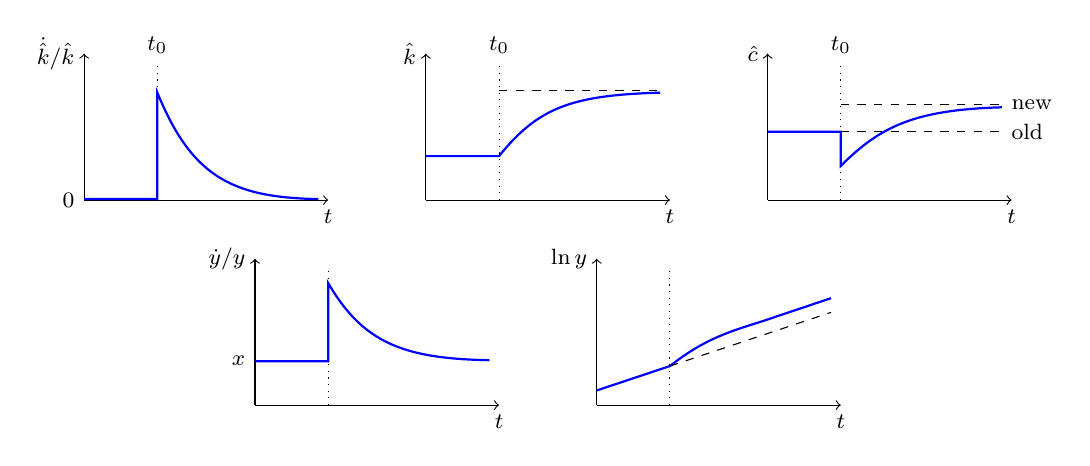
\begin{tikzpicture}[scale=0.62,every node/.style={font=\footnotesize}]
% row 1
\draw[->](0,0)--(5,0) node[below]{$t$}; \draw[->](0,0)--(0,3) node[left]{$\dot{\hat k}/\hat k$};
\draw[dotted](1.5,0)--(1.5,2.8) node[above]{$t_0$}; \node[left] at (0,0){$0$};
\draw[thick,blue](0,0.02)--(1.5,0.02)--(1.5,2.2) .. controls (2.2,0.5) and (3,0.05) .. (4.8,0.02);
\begin{scope}[shift={(7,0)}]
\draw[->](0,0)--(5,0) node[below]{$t$}; \draw[->](0,0)--(0,3) node[left]{$\hat k$};
\draw[dotted](1.5,0)--(1.5,2.8) node[above]{$t_0$};
\draw[thick,blue](0,0.9)--(1.5,0.9) .. controls (2.3,1.9) and (3,2.15) .. (4.8,2.2);
\draw[dashed](1.5,2.25)--(4.8,2.25);
\end{scope}
\begin{scope}[shift={(14,0)}]
\draw[->](0,0)--(5,0) node[below]{$t$}; \draw[->](0,0)--(0,3) node[left]{$\hat c$};
\draw[dotted](1.5,0)--(1.5,2.8) node[above]{$t_0$};
\draw[thick,blue](0,1.4)--(1.5,1.4)--(1.5,0.7) .. controls (2.3,1.5) and (3,1.85) .. (4.8,1.9);
\draw[dashed](1.5,1.4)--(4.8,1.4) node[right]{old};
\draw[dashed](1.5,1.95)--(4.8,1.95) node[right]{new};
\end{scope}
% row 2
\begin{scope}[shift={(3.5,-4.2)}]
\draw[->](0,0)--(5,0) node[below]{$t$}; \draw[->](0,0)--(0,3) node[left]{$\dot y/y$};
\draw[dotted](1.5,0)--(1.5,2.8); \node[left] at (0,0.9){$x$};
\draw[thick,blue](0,0.9)--(1.5,0.9)--(1.5,2.5) .. controls (2.2,1.3) and (3,0.95) .. (4.8,0.92);
\end{scope}
\begin{scope}[shift={(10.5,-4.2)}]
\draw[->](0,0)--(5,0) node[below]{$t$}; \draw[->](0,0)--(0,3) node[left]{$\ln y$};
\draw[dotted](1.5,0)--(1.5,2.8);
\draw[thick,blue](0,0.3)--(1.5,0.8) .. controls (2.2,1.35) and (2.7,1.5) .. (3.4,1.72)--(4.8,2.19);
\draw[dashed](1.5,0.8)--(4.8,1.9);
\end{scope}
\end{tikzpicture}
\end{center}
\textbf{How to read the panels.} Top row: growth of $\hat k$ (jumps, then decays to $0$), the level of $\hat k$ (rises smoothly to the higher SS), and consumption $\hat c$ (drops at $t_0$, then overshoots the old level). Bottom row: $\dot y/y$ (jumps above $x$, then returns to $x$) and $\ln y$, whose slope is $\dot y/y$. The dashed line in the $\ln y$ panel is the old path: the new path is steeper for a while and then runs parallel to it at a higher level.

\begin{tipbox}
In the Solow model a change in $s$ (or in the level of $A$) never changes the long-run growth rate of $y$; only $x$ does. Always draw $\ln y$ returning to slope $x$, parallel to the old path.
\end{tipbox}

%=====================================================================
\subsection{Application: foreign aid \pg{7}}

\paragraph{Setup.} A poor country is described by \eqref{eq:sol-fund}. Let ``aid'' denote the amount of aid per effective worker, received each period (a constant). Compare four forms of aid.

\begin{enumerate}
  \item \textbf{Consumption goods.} The aid is consumed directly:
  \[
  \hat c_t=(1-s)\hat k_t^{\alpha}+\text{aid},\qquad \dot{\hat k}_t=s\hat k_t^{\alpha}-(\delta+n+x)\hat k_t\ \ \text{(unchanged)}.
  \]
  The accumulation equation is unaffected, so the aid has no effect on the factors of production ($\hat k$, $\hat k^*$ and $\hat y$ are unchanged). It provides only temporary relief: more aid will be required in the future. It may still be necessary (e.g.\ famine relief) even though it is not a lasting solution.
  \item \textbf{Capital goods (a one-time transfer of capital).} Poor countries have low $\hat k$, so they are far below their SS. A transfer of capital raises $\hat k$ immediately, moving the economy to the right along the $\hat k$ axis in the phase diagram, and so speeds up the development process. The gain is lasting in the sense that it does not need to be repeated: the country is permanently further along its transition. But $\hat k^*$ in \eqref{eq:sol-kss} is unchanged, so the long-run path of $y$ is the same.
  \item \textbf{Technical assistance ($A\uparrow$).} Poor countries also have low technology levels. As in the one-time rise in $A$ above: the \emph{direct} effect raises $y$ immediately; the \emph{indirect} effect lowers $\hat k=K/(AL)$, pushing the economy back into transitional growth, so capital accumulation starts again. Long-run $y$ is permanently higher.
  \item \textbf{Money.} Money is not capital: the country treats the aid as extra income, saves only the fraction $s$ of it and consumes the rest. Investment per effective worker becomes $\hat i_t=s(\hat k_t^{\alpha}+\text{aid})$, so
  \begin{equation}\label{eq:sol-aid}
  \dot{\hat k}_t=s\hat k_t^{\alpha}+s\cdot\text{aid}-(\delta+n+x)\hat k_t .
  \end{equation}
\end{enumerate}

\paragraph{Effect of money aid on the steady state.} The new SS $\hat k^{ss}_{new}$ solves $s(\hat k^{\alpha}+\text{aid})=(\delta+n+x)\hat k$.
\begin{itemize}
  \item At the old SS $\hat k^{ss}$, $s(\hat k^{ss})^{\alpha}=(\delta+n+x)\hat k^{ss}$, so \eqref{eq:sol-aid} gives $\dot{\hat k}=s\cdot\text{aid}>0$: $\hat k$ starts to rise, and $\hat k^{ss}_{new}>\hat k^{ss}$.
  \item Implicit function theorem (if $F(\hat k,a)=0$ then $d\hat k/da=-F_a/F_{\hat k}$) with $F=s\hat k^{\alpha}+s\,a-(\delta+n+x)\hat k$ and $a=\text{aid}$:
  \[
  \frac{d\hat k^{ss}_{new}}{d\,\text{aid}}=\frac{s}{(\delta+n+x)-s\alpha\hat k^{\alpha-1}} .
  \]
  The denominator is positive: at the new SS, $(\delta+n+x)\hat k=s\hat k^{\alpha}+s\cdot\text{aid}>s\hat k^{\alpha}$, so $\delta+n+x>s\hat k^{\alpha-1}>s\alpha\hat k^{\alpha-1}$. Hence the effect is positive, and it is proportional to $s$.
\end{itemize}
\textit{Interpretation:} the effectiveness of money aid in raising $\hat k$ depends in part on $s$. If the fraction of the aid money that is saved is low, it does little for capital accumulation; most of it simply raises consumption, as in case 1.

\begin{center}
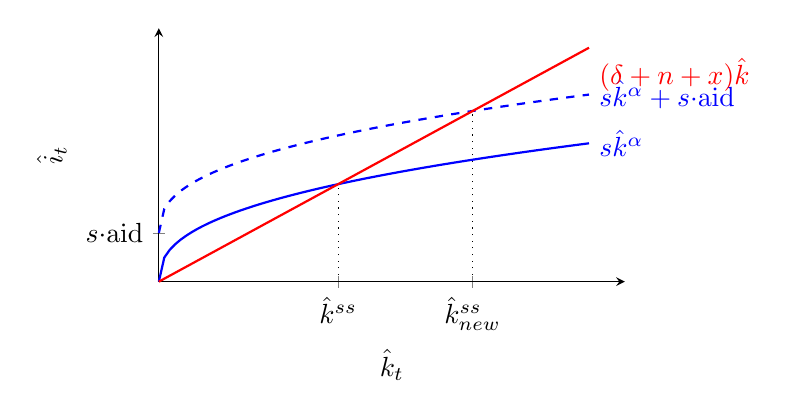
\begin{tikzpicture}
\begin{axis}[width=7.5cm,height=4.8cm,axis lines=left,xmin=0,xmax=2.6,ymin=0,ymax=1.3,
  xtick={1,1.75},xticklabels={$\hat k^{ss}$,$\hat k^{ss}_{new}$},ytick={0.25},yticklabels={$s\cdot$aid},
  xlabel={$\hat k_t$},ylabel={$\hat i_t$},clip=false]
\addplot[thick,blue,domain=0:2.4,samples=80]{0.5*x^0.4} node[right]{$s\hat k^{\alpha}$};
\addplot[thick,blue,dashed,domain=0:2.4,samples=80]{0.25+0.5*x^0.4} node[right]{$s\hat k^{\alpha}+s\cdot$aid};
\addplot[thick,red,domain=0:2.4]{0.5*x} node[below right]{$(\delta+n+x)\hat k$};
\draw[dotted](axis cs:1,0)--(axis cs:1,0.5); \draw[dotted](axis cs:1.75,0)--(axis cs:1.75,0.875);
\end{axis}
\end{tikzpicture}
\end{center}
\textbf{How to read the diagram.} Money aid shifts the investment curve up by the constant $s\cdot\text{aid}$, so the dashed curve starts at the intercept $s\cdot\text{aid}$ on the vertical axis. It crosses the unchanged break-even line further to the right, at $\hat k^{ss}_{new}$. The smaller $s$ is, the smaller the upward shift and the smaller the gain in $\hat k^{ss}$.

%=====================================================================
\subsection{Solow model with land and natural resources \pg{9--10}}

\paragraph{Question.} How would a fixed factor (land) and a non-renewable resource affect the long-run growth rate of an economy?

\paragraph{Setup.}
\begin{itemize}
  \item Inputs: capital $K_t$, effective labour $A_tL_t$, a non-renewable natural resource $R_t$ (the amount used in production each period), and land $T_t$.
  \item Growth assumptions: $\dot L_t/L_t=n$, $\dot A_t/A_t=x$, $\dot R_t/R_t=-b$ with $b>0$ (the resource input shrinks at rate $b$ as it is depleted), $\dot T_t=0$ (land is fixed).
  \item Exponents $\alpha,\beta,\gamma>0$ with $\alpha+\beta+\gamma<1$; effective labour gets exponent $1-\alpha-\beta-\gamma>0$, so production has constant returns in all four inputs.
  \item Saving rule and depreciation as before: $I_t=sY_t$, depreciation rate $\delta$.
\end{itemize}
\begin{align}
Y_t&=(A_tL_t)^{1-\alpha-\beta-\gamma}K_t^{\alpha}R_t^{\beta}T_t^{\gamma}, \label{eq:sol-lr1}\\
\dot K_t&=I_t-\delta K_t=sY_t-\delta K_t\ \Longrightarrow\ \frac{\dot K_t}{K_t}=s\frac{Y_t}{K_t}-\delta \quad\text{(divide by $K_t$)}. \label{eq:sol-lr2}
\end{align}

\paragraph{Growth rate of output.} Take logs of \eqref{eq:sol-lr1}:
\[
\ln Y_t=(1-\alpha-\beta-\gamma)(\ln A_t+\ln L_t)+\alpha\ln K_t+\beta\ln R_t+\gamma\ln T_t .
\]
Differentiate with respect to $t$, using $d\ln X/dt=\dot X/X$:
\begin{align*}
\frac{\dot Y_t}{Y_t}&=(1-\alpha-\beta-\gamma)\Big(\frac{\dot A_t}{A_t}+\frac{\dot L_t}{L_t}\Big)+\alpha\frac{\dot K_t}{K_t}+\beta\frac{\dot R_t}{R_t}+\gamma\frac{\dot T_t}{T_t}\\
&=(1-\alpha-\beta-\gamma)(x+n)+\alpha\frac{\dot K_t}{K_t}+\beta(-b)+\gamma\cdot 0 .
\end{align*}
\begin{equation}\label{eq:sol-lr3}
\frac{\dot Y_t}{Y_t}=(1-\alpha-\beta-\gamma)(x+n)-\beta b+\alpha\frac{\dot K_t}{K_t}.
\end{equation}

\paragraph{Balanced growth path (BGP).} Suppose a BGP exists on which $Y$ and $K$ grow at the same constant rate $g$. (This is the only possibility with constant growth: by \eqref{eq:sol-lr2}, constant $\dot K/K$ requires constant $Y/K$, i.e.\ $\dot Y/Y=\dot K/K$.) Set $\dot Y/Y=\dot K/K=g$ in \eqref{eq:sol-lr3}:
\begin{align*}
g&=(1-\alpha-\beta-\gamma)(x+n)-\beta b+\alpha g\\
(1-\alpha)g&=(1-\alpha-\beta-\gamma)(x+n)-\beta b && \text{(move $\alpha g$ to the left)}
\end{align*}
\begin{equation}\label{eq:sol-lr4}
g=\Big[\frac{1-\alpha-\beta-\gamma}{1-\alpha}\Big](x+n)-\Big[\frac{\beta}{1-\alpha}\Big]b \qquad\text{(divide by $1-\alpha>0$)}.
\end{equation}

\paragraph{Does the economy converge to the BGP?} Yes. Subtract \eqref{eq:sol-lr4}, written as $g=(1-\alpha-\beta-\gamma)(x+n)-\beta b+\alpha g$, from \eqref{eq:sol-lr3}; the constant terms cancel:
\begin{equation}\label{eq:sol-lr5}
\frac{\dot Y_t}{Y_t}-g=\alpha\Big(\frac{\dot K_t}{K_t}-g\Big).
\end{equation}
Recall from \eqref{eq:sol-lr2} that $\dot K/K$ moves in the same direction as $Y/K$, and $Y/K$ rises when $\dot Y/Y>\dot K/K$ and falls when $\dot Y/Y<\dot K/K$.
\begin{itemize}
  \item[(i)] $\dot K/K>g$. By \eqref{eq:sol-lr5} the RHS is positive, so $\dot Y/Y>g$. But since $\alpha<1$, $\dot Y/Y-g<\dot K/K-g$, i.e.\ $\dot Y/Y<\dot K/K$. So $Y/K$ falls during the transition, and by \eqref{eq:sol-lr2} $\dot K/K$ falls toward $g$.
  \item[(ii)] $\dot K/K<g$. By \eqref{eq:sol-lr5}, $\dot Y/Y<g$, and since $\alpha<1$, $\dot Y/Y>\dot K/K$. So $Y/K$ rises, and by \eqref{eq:sol-lr2} $\dot K/K$ rises toward $g$.
  \item[(iii)] $\dot K/K=g$. By \eqref{eq:sol-lr5}, $\dot Y/Y=g$, so $Y/K$ is constant and $\dot K/K$ stays at $g$.
\end{itemize}
\textit{Conclusion:} from (i)--(iii), the economy moves toward the BGP regardless of initial conditions, and once it reaches the BGP it remains there.

\paragraph{Long-run growth of per-capita variables.} All per-capita variables (e.g.\ $y=Y/L$, $k=K/L$) grow at $g-n$. Subtract $n$ from \eqref{eq:sol-lr4}:
\begin{align*}
g-n&=\frac{(1-\alpha-\beta-\gamma)(x+n)-\beta b-(1-\alpha)n}{1-\alpha} && \text{(common denominator)}\\
&=\frac{(1-\alpha-\beta-\gamma)x+\big[(1-\alpha-\beta-\gamma)-(1-\alpha)\big]n-\beta b}{1-\alpha} && \text{(collect $n$)}\\
&=\frac{(1-\alpha-\beta-\gamma)x-(\beta+\gamma)n-\beta b}{1-\alpha} .
\end{align*}
\begin{keybox}[title=Long-run per-capita growth with land and resources]
\begin{equation}\label{eq:sol-lr6}
g-n=\underbrace{\Big[\frac{1-\alpha-\beta-\gamma}{1-\alpha}\Big]x}_{(a)}-\underbrace{\Big[\frac{\beta}{1-\alpha}\Big]b}_{(b)}-\underbrace{\Big[\frac{\beta+\gamma}{1-\alpha}\Big]n}_{(c)}
\end{equation}
\begin{itemize}
  \item (b) \textbf{Resource depletion:} the resource is being used up, so less is available each period. This adversely affects production, and growth slows.
  \item (c) \textbf{Congestion:} with a depletable resource and a fixed factor, population growth means each worker has less land and less resource to work with. This congestion slows per-capita growth.
  \item (a) \textbf{Technology:} $g-n$ can still be positive if $x$ is sufficiently large, precisely if $(1-\alpha-\beta-\gamma)x>\beta b+(\beta+\gamma)n$. Technological progress can outrun depletion and congestion.
\end{itemize}
\end{keybox}
\textit{Check:} with no land and no resource ($\beta=\gamma=0$), \eqref{eq:sol-lr6} reduces to $g-n=x$, the standard Solow result (fact 1).
